\documentclass[10pt, a4paper,spanish]{article}
\usepackage[utf8]{inputenc}

\usepackage{hyperref}

\usepackage[T1]{fontenc}

\usepackage[hmarginratio=1:1,top=32mm,columnsep=20pt]{geometry}
\usepackage[hang, small,labelfont=bf,up,textfont=it,up]{caption}


\usepackage{graphicx}
\graphicspath{ {images/} }

\usepackage{abstract}
\renewcommand{\abstractnamefont}{\normalfont\bfseries}
\renewcommand{\abstracttextfont}{\normalfont\small\itshape}

\usepackage{titlesec}
\renewcommand\thesection{\Roman{section}}
\renewcommand\thesubsection{\Roman{subsection}}
\titleformat{\section}[block]{\large\scshape\centering}{\thesection.}{1em}{}
\titleformat{\subsection}[block]{\large}{\thesubsection.}{1em}{}


\usepackage{fancyhdr}
\pagestyle{fancy}
\fancyhead{}
\fancyfoot{}
\fancyhead[C]{ \today \ $\bullet$ Minería de Datos $\bullet$ Multicomparación de Clasificadores}
\fancyfoot[RO]{\thepage}

%-------------------------------------------------------------------------------
%	TITLE SECTION
%-------------------------------------------------------------------------------

\title{\vspace{-15mm}\fontsize{24pt}{10pt}\selectfont\textbf{Multicomparación de \\ Clasificadores}} % Article title

\author{Sergio García Prado}
\date{\today}

%-------------------------------------------------------------------------------

\begin{document}

	\maketitle % Insert title

	\thispagestyle{fancy} % All pages have headers and footers

%-------------------------------------------------------------------------------
%	ABSTRACT
%-------------------------------------------------------------------------------

	\begin{abstract}
		\noindent
	\end{abstract}

%-------------------------------------------------------------------------------
%	TEXT
%-------------------------------------------------------------------------------

	\section{Introducción}

        \paragraph{}
		La comparación consistirá en dos partes principales: la primera de ellas se basa en un Test de Signos sobre 2 de los clasificadores para todos los conjuntos de datos, mientras que la segunda parte se refiere a la realización de un Ranking en el cuál participarán todos los clasificadores.

		\paragraph{}
		Para la realización de estas pruebas se ha utilizado Weka, que es una plataforma de software para el aprendizaje automático y la minería de datos escrita en Java, desarrollada en la Universidad de Waikato y distribuida como Software Libre.

		\paragraph{}
		Por lo tanto, lo primero es describir tanto los clasificadores como los conjuntos de datos que se utilizarán en los tests de clasificación:

		\subsection{Clasificadores}

			\begin{itemize}
				\item \textbf{SVM con kernel lineal}:
				\item \textbf{3-NN}:
				\item \textbf{Naive Bayes}:
				\item \textbf{J48}:
			\end{itemize}

		\subsection{Conjuntos de Datos}

			\begin{enumerate}
				\item \textbf{Arrhythmia}:
				\item \textbf{Diabetes}:
				\item \textbf{Glass}:
				\item \textbf{Ionosphere}:
				\item \textbf{Iris}:
				\item \textbf{Labor}:
				\item \textbf{Seeds}:
				\item \textbf{Segment Test}:
				\item \textbf{Soybean}:
				\item \textbf{Vote}:
			\end{enumerate}


	\section{Test de Signos: SVM y J48}

        \paragraph{}
		El test de signos se ha realizado sobre los 10 conjuntos de datos aplicando validación cruzada de 10 particiones. Lo que se pretende con este test es contar el número de victorias de cada clasificador y otorgarle la victoria al que más número de veces haya sido seleccionado ganador. Los resultados obtenidos han sido los siguientes:

		\hfill
		\begin{center}
			\begin{tabular}{ | c || c | c | c | c | c | c | c | c | c | c | }
				\hline
				Datos		& 1 	& 2		& 3 	& 4 	& 5 	& 6		& 7 	& 8 	& 9 	& 10 \\ \hline \hline
				Ganador		& SVM 	& SVM 	& J48 	& J48 	& SVM 	& SVM 	& SVM 	& J48 	& SVM 	& J48 \\
				\hline
			\end{tabular}
		\end{center}

		\paragraph{}
		Por lo tanto, los resultados de aplicar el test de signos son los siguientes:
		\[Victorias(J48) = 4\]
		\[Victorias(SVM) = 6\]
		Entonces podemos concluir que para los conjuntos de datos utilizados, obtiene más victorias, por lo tanto en promedio genera mejores resultados, el clasificador \textbf{SVM}.

	\section{Ranking}

        \paragraph{}
		\begin{center}
			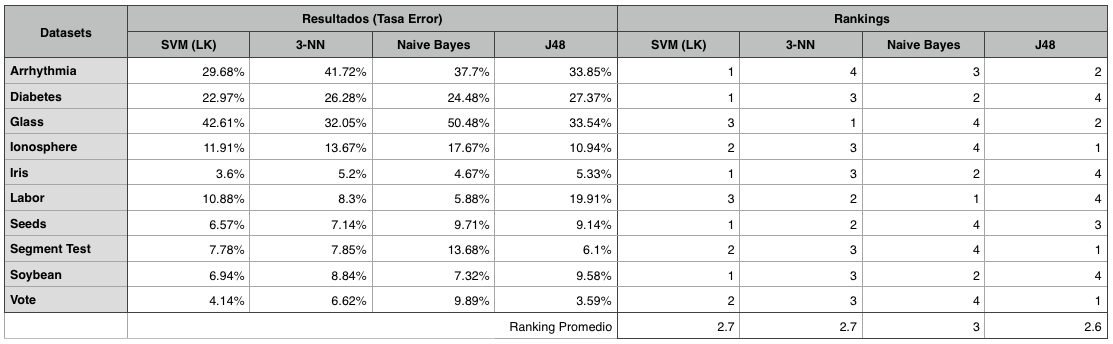
\includegraphics[width=\textwidth]{ranking-table}
		\end{center}

		$K = 4$, $N =10$,
		$K-1 = 3$,$N-1 =9$,
		$(k-1)(N-1) = 27$
		$\alpha = 0.05$
		$F_{3,27} =  2.960$
\end{document}
